% !TeX root = ../main.tex

\chapter{绪论}

\section{研究的背景及意义}

\subsection{分布式事务模型}
  事务是计算机数据库领域中的一个重要的概念,事务的存在确保了系统能够按照应用开发者既定的逻辑完成工作,并承担了错误恢复、错误处理的功能。简单的说,事务就是恢复和并发控制的基本单位,是用户定义的一个操作序列,在单个逻辑工作中执行一系列的操作,要么全部执行,要么全部不执行。

  事务应该具有4个属性:原子性(atomicity)、一致性(consistency)、隔离性(isolation)、持久性(durability)。原子性申明了事务的不可分割的特点,一致性指数据库一致地从一个一致性状态转移到另一个一致性状态,隔离性定义为一个事务的执行不能被其他事务干扰,即一个事务内部的操作及使用的数据对并发的其他事务是隔离的,而耐久性则提供了一个事务一旦被提交,它对数据库中数据的改变是永久性的特点,即接下来的操作或故障不应该对其有任何影响。

  传统数据库历经了几十年的发展,对事务的ACID性质都有了很好的保证,并最大程度的优化了系统的性能。但随着信息时代的不断发展,数据不断膨胀,单点机器很难再满足用户的需求。为了避免单点故障或是单点机器的性能瓶颈问题,开发者往往将数据分成多个数据块并将它们储存在不同的机器上。同时,为了避免物理破坏,代码漏洞等问题带来的数据损坏,开发者还往往会对数据存有多个备份。在这样的背景下,分布式事务氤氲而生。
  
  一个典型的可拓展的且提供容错备份的分布式数据库的结构如下图所示:

\begin{figure}[htb]
  \centering
  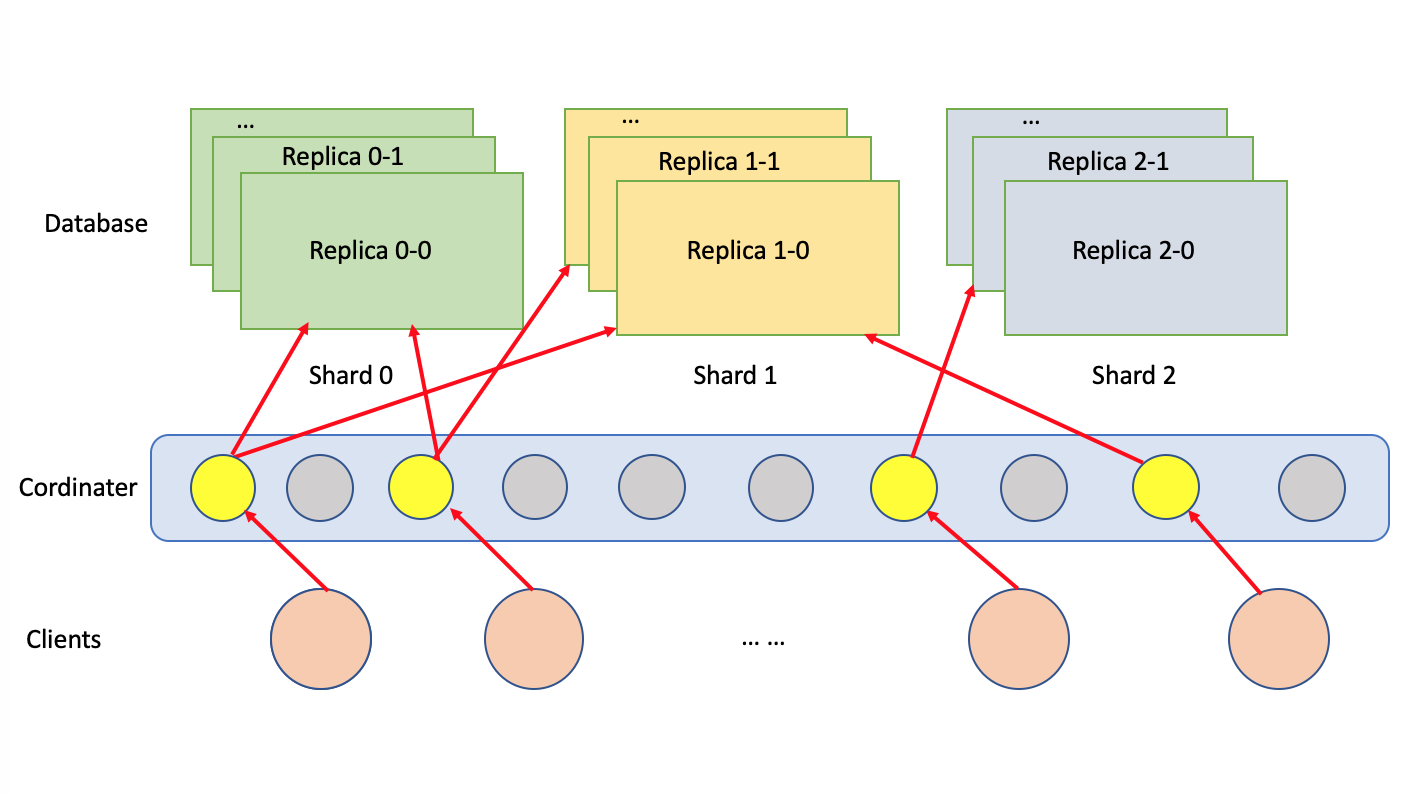
\includegraphics[width=0.76\textwidth]{Distributed_Txn.png}
  \caption{分布式事务模型}
  \label{fig:badge}
\end{figure}


  分布式事务不仅仍需要保证ACID的性质,还要处理跨机器,跨数据库中间的协同问题。\cite{MultiDBTXN1,MultiDBTXN2,MultiDBTXN3}为了解决分布式事务中的协同问题,不失一般性的,我们通常会有一个事务的组织者(coordinator)和事务的参与者(participants)。事务的组织者负责通知参与者,协同他们的工作,使得不同的参与者能够最终得到相同的事务处理结果,即提交或放弃。比较经典的分布式事务提交协议包括了:两阶段提交协议(2-Phase-Commit)、TCC(Try, Confirm, Cancel)等。
  
  以二阶段提交为例,分为第一阶段:投票阶段和第二阶段:执行阶段。用户(client)向组织者(coordinator)发起事务请求,组织者负责根据事务的内容选定组织者。在事务的提交阶段,组织者先向所有的参与者发起投票请求,即询问参与者是否已经做好了提交准备,参与者收到请求后,将投票决定写入磁盘,并回复组织者,直至得到所有参与者肯定的答复或者至少一个参与者否定答复后,协议进入第二阶段,组织者将信息相关信息写入磁盘,并向所有参与者发起提交(Commit)或放弃(Abort)请求,参与者在收到请求后需要执行相关操作,并将决定写入磁盘,最后回复组织者。直至所有参与者回复了已经提交的答复,事务才算真正完成。
  
  \begin{figure}[htb]
  \centering
  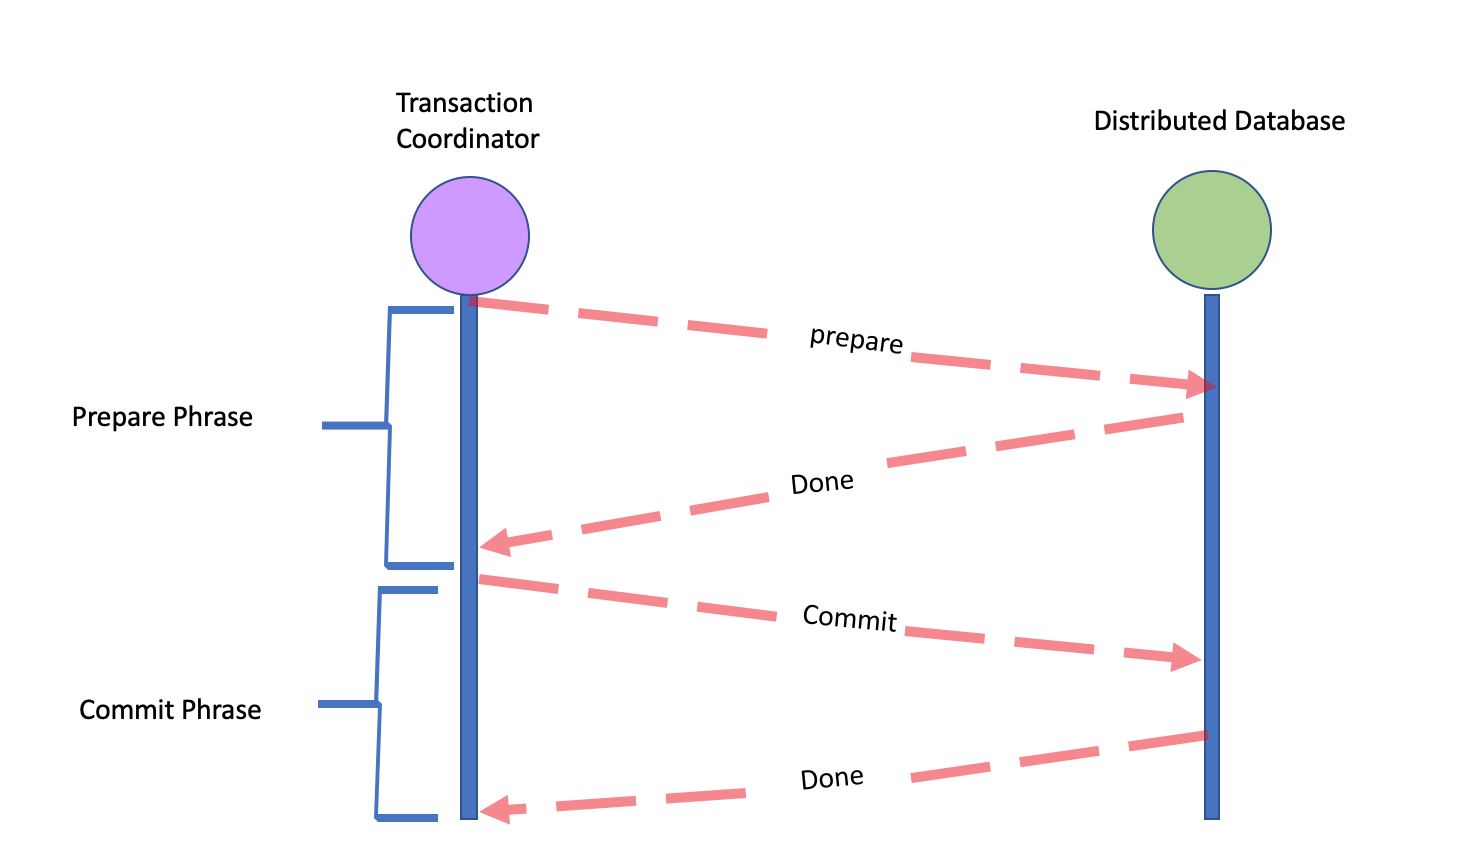
\includegraphics[width=0.76\textwidth]{2PC.png}
  \caption{2阶段提交协议}
  \label{fig:badge}
\end{figure}

  值得注意的是协议的设计保证了,系统在任何的一个时刻奔溃,都能恢复到正确的结果。试想,如果在提交阶段,我们仍然采用单机的提交协议,而不事先询问投票会发生什么呢?此时,如果其中一个参与者选择放弃提交,那么参与者之间将会出现歧义(对于同一事务,同时存在提交或不提交的参与者),使得系统不一致。永久化操作也保证了,所有参与者或组织者在宕机后,重启时,都能够有效地看到宕机前的处理结果,从而保证事务的正确执行。



\subsection{异地冗余存储系统的发展}
  冗余是为了更好的实现容错,在系统崩溃时,使用者可以使用备份来替换原有的损坏的机器,从而提供更加稳定的服务。\cite{Spanner}你可能会认为,我的个人电脑工作得很好,一年也不一定会坏,那还有必要实现容错吗?事实上,对于一个巨大的集群,或数据中心,错误时时刻刻都在发生。这从概率上可以很容易的得到解释,假设
  一台机器每一年坏一次,那么当你拥有1000台机器时,几乎每几个小时都有机器处于错误状态。所以如果你拥有成百上千的服务器,容错就成了无法避免的话题,出错将是发生的常态,而不是偶然。一般而言,冗余能够帮助解决单点错误,比如:风扇停止转动、CPU过载、软件错误导致的关机、网路链接中断、磁盘错误、断电等。


  但对于位于同一地点的备份(例如:备份位于同一数据中心内),备份并没有办法在所有备份同时被破坏时实现容错。比如:突如其来的洪水、地震、地域性停电等。有一些系统对容错的等级要求较高,例如:银行交易系统、股票交易系统等。试想:如果某地发生地震导致所有某银行的所有用户的数据丢失,那简直是一场比地震更可怕的灾难。在这一背景下,异地冗余的方案被人们所接受。

  异地冗余不仅带来了更高的容错等级,同时还为系统性能的优化提供了可能。异地冗余使得数据源与用户的距离更近,从而使得用户可以更快地访问数据,特别是对于读取任务。譬如:一个中国用户,想访问存在美国的数据库中的数据,如果这个数据库在中国存在一个异地的备份,那么用户将不用通过跨大陆的海底光缆来获得数据,而只需要访问中国的备份数据来完成读取任务。这种地区性的读取访问优化,对于许多实际场景来说是广泛试用的,因为在需要工作任务中,读取事务所占的比例比更新和修改事务多得多。
 
 \begin{figure}[htb]
  \centering
  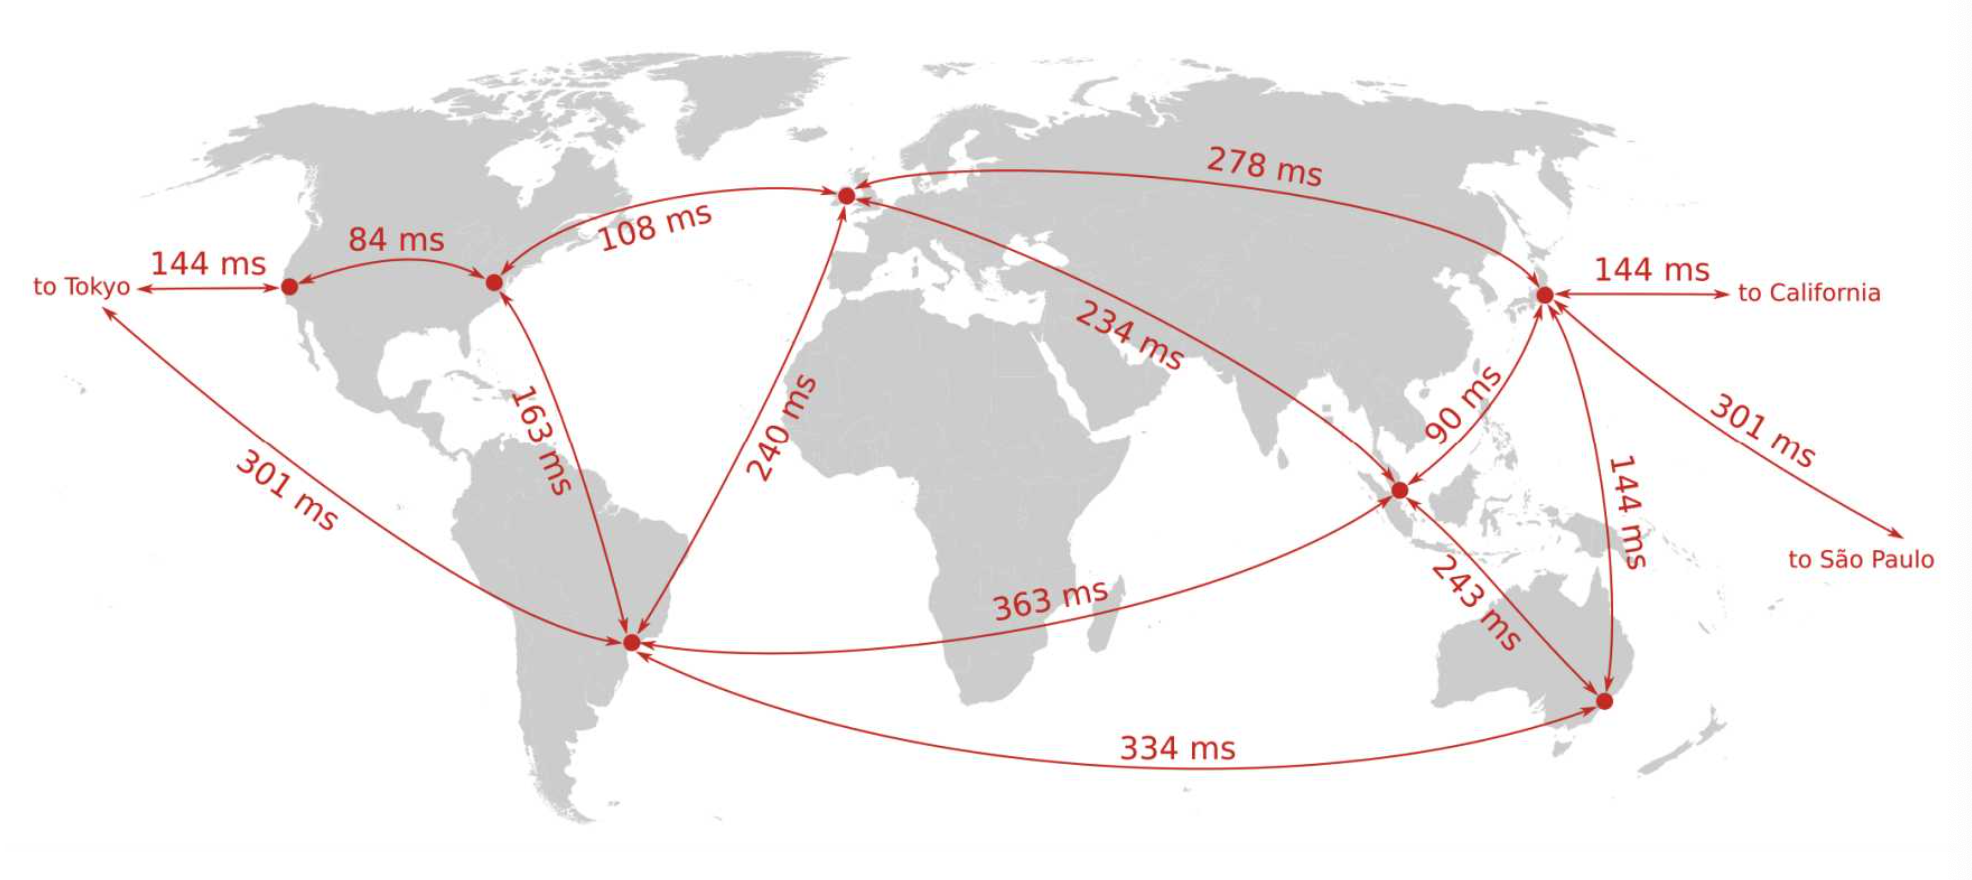
\includegraphics[width=0.86\textwidth]{DC.png}
  \caption{分布在全球的数据中心}
  \label{fig:badge}
\end{figure}

  随着云计算时代的到来,异地冗余备份面临了更多的可能。中小企业不需要在世界各地花费巨额建立属于自己的数据中心,就能够享受到同等的服务。诸多云计算服务提供商,例如:微软、谷歌、亚马逊;都提供了遍布地球的数据中心服务,用户可以简单地租赁不同数据中心的服务器来搭建自己的系统。
  
  当然,异地冗余系统也带来了巨大的副本同步问题,面临着巨大的挑战。原本在同一个数据中心内,主体与副本的同步开销到了异地背景下,被夸张的放大了,主体与副本之间通讯的时延从零点几微秒到了几百微妙。因此,在这一环境下,设计一个好的同步方式尤为重要,尽可能地减少跨数据中心的协同合作,成为了设计的主要目标。


\subsection{强一致性(线性一致性)}
 数据的一致性指数据的多个副本之间保持一致的特性。

 在数据有多份副本的情况下,如果网络、服务器或者软件出现故障,会导致部分副本写入成功,部分副本写入失败。这就造成各个副本之间的数据不一致,数据内容冲突。而强一致性要求:当更新操作完成之后,任何多个后续进程或者线程的访问都会返回最新的更新过的值。这种是对用户最友好的,就是用户上一次写入什么,下一次就保证能读到什么。那么为什么我们希望实现强一致性的系统呢?

 分布式系统的一个设计原则是尽可能向用户或应用开发者提供看起来像一台机器的服务,也就是说,无论分布式系统背后有多少工作的机器,有多复杂的设计架构,用户可以像使用单台机器一样使用和调度集群。这样的设计使得分布式系统易于使用,降低了使用门槛,使得其适用于范围更加广泛的产品。

 正是由于这样简洁而有简单的愿望,强一致性成了科研人员和企业所青睐的选择。一般根据数据库的一致性要求,有以下几种一执性模型:强一致性、弱一致性、最终一致性、读写一致性、因果一致性。而强一致性模型则是其中最强的,也就是线性一执性模型。在该模型中,所有的事务被线性化,使得分布式系统能够像单个机器一样提供服务。它保持副本与主体的完全一致性,使得在所有在主体上完成的事务,在副本上都可见。虽然其他的一致性模型,也被许多系统所广泛采用。但他们要么能够忍受读取奇怪的结果(比如:读取副本时,陈旧的数据),要么需要应用开发者精心的设计。

 强一致性的愿景是美好的,但是往往比其他一执行模型需要付出更大的代价。以最简单的强一致性实现方法为例,在确定性集群(给定初始状态和确定性的执行,机器能够执行并得到相一致的最终状态)中,为了保证副本和主体执行完全相同的序列,我们需要将不同用户发出事务进行序列化,因此我们需要一个中心节点来完成。中心节点存在的问题是显而易见的,首先是单个中心节点容易收到攻击或出错,其次中心节点容易成为性能瓶颈。因此,人们设计了许多分布式序列化的方法,比如Paxos、Raft等协议。这使得这一问题稍微缓解,但代价却是昂贵的,这些协议都需要多个RTT来完成协议内容,使系统变差。同时,其本身还带来了吞吐量的限制。

 目前,广泛使用的实现强一致性的方法,主要可以分为两类:

\begin{itemize}
\item 将所有事务进行全序化
\item 只计算冲突事务的偏序集合
\end{itemize}


\subsection{并发控制简述}

并发控制是指在多个用户、进程或线程同时对数据库进行操作时,保证事务的一致性和隔离性。同时最大程度地并发,提高系统的吞吐量。并发控制的目的是保证一个用户的工作不会对另一个用户的工作产生不合理的影响。在某些情况下,这些措施保证了当用户和其他用户一起操作时,所得的结果和单独操作时的结果保持一致。
被广泛使用的并发控制协议,大致可以分为两个流派:

\begin{itemize}
\item 悲观并发控制协议(Pessimistic Concurrency Control)
\item 乐观并发控制协议 (Optimistic concurrency control)
\end{itemize}
下面简单介绍两种并发控制具有代表性的方法,并分析各自的利弊。

\paragraph{悲观并发控制协议}

悲观方法适用于数据访问冲突频率较高的情况,其基本思想是使一个产生冲突的事务处于等待状态,直到冲突消解后,处于等待状态的事务才能够继续执行。一般使用锁机制来实现悲观控制协议。其中二阶段锁(Two-Phase-Lock)是保证事务可被串行化的充分条件,并且在没有额外的抽象语义的条件下,还是必要条件。

二阶段锁的基本原则是在同一个事务内,对所涉及的所有数据项进行先加锁,然后才对所有的数据项解锁。如下图所示:
  \begin{figure}[htb]
  \centering
  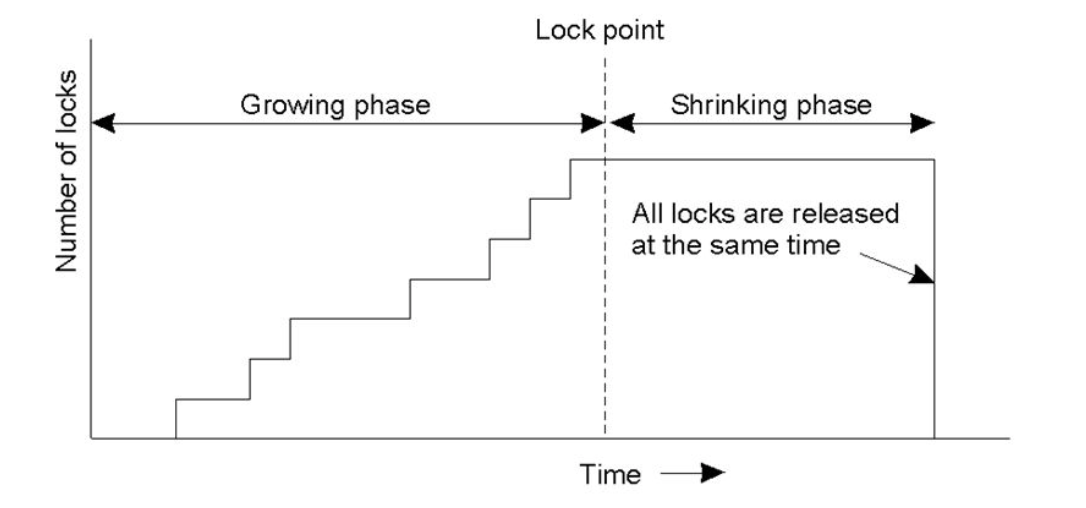
\includegraphics[width=0.76\textwidth]{2PL.png}
  \caption{2阶段锁}
  \label{fig:badge}
\end{figure}

基本的二阶段锁会产生死锁问题,通常采用放弃事务的方法来消除死锁。可以严格约定在事务提交或放弃后再释放锁,但这是以牺牲部分并发度为代价的。

\paragraph{乐观并发控制协议}

乐观控制是一种并发程度更高的控制协议\cite{OCC},适用于数据访问冲突频率较低的情况。乐观控制允许事务不提前检查冲突,而是使得相互冲突的事务继续运行,直到事务提交时,系统才对事务进行有效性验证。经典的做法是,系统在事务开始运行时都会赋予每个事务一个时间戳,事务在其生存期内应该对数据库有一个一致的视图。在事务提交时,系统根据附带的时间戳,对视图的一致性进行检查,若检查通过,则事务可以提交。否则就放弃。

经典的乐观并发控制如下图所示:
 
\begin{figure}[htb]
  \centering
  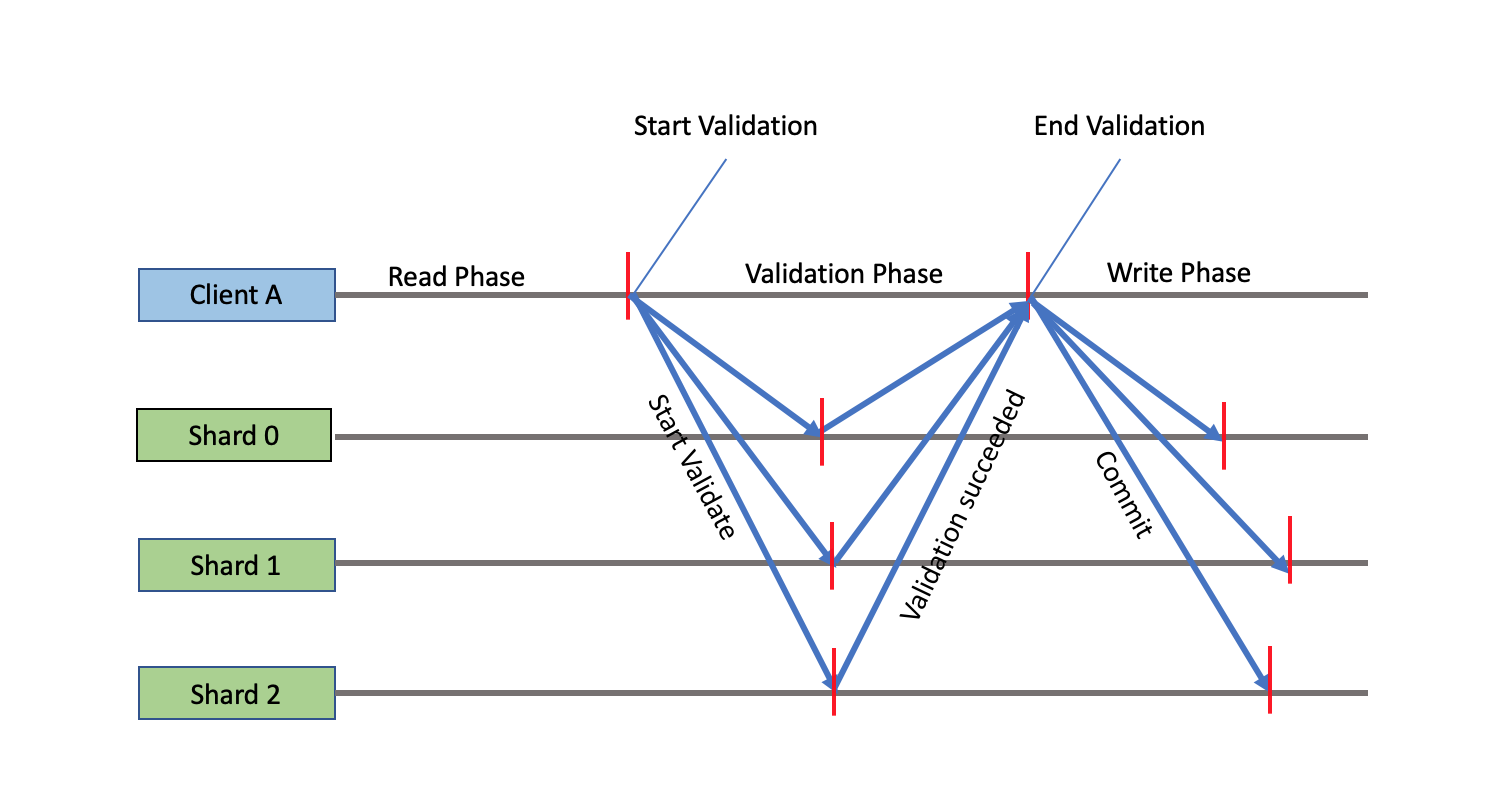
\includegraphics[width=0.96\textwidth]{OCC.png}
  \caption{乐观控制协议}
  \label{fig:badge}
\end{figure}

乐观控制的方法只在提交阶段进行加锁(避免两个事务同时提交)并进行有效性验证,这提高了并发度,但在数据访问冲突频繁的情况下,事务的放弃率(Abort Rate)会很高。

\subsection{研究的意义}

异地冗余的存储系统为提供更高的容错等级和支持快速的远程数据访问提供了可能,但却因为因为其高昂的写入代价而被人们所诟病。优化实现基于异地冗余存储系统的并发控制和共识机制的实现,为进一步商业推广使用异地冗余系统提供了可能。也进一步优化了,既有系统的性能,包括延时和吞吐量。



\section{研究的目标及主要工作}

本文的目标是整理近年来对异地冗余存储系统的并发控制和共识协议的优化设计,并在此基础上分析他们在不同负载下的表现,并对系统进行复现和调优。同时归纳这些工作的不足之处,达到抛砖引玉的效果。

主要工作如下:

(1)在Janus的codebase 上实现Ocean Vista 和SLOG 使得多个系统能够在同一代码框架下进行较为公平的性能比较。并在不同的负载下,比较各个系统的性能差异,以及各系统设计的特点。

(2)优化基准测试集TPCC的实现,使其更好地支持one-shot事务。具体表现为通过垂直划分,将部分只读数据备份到所有机器上。这将使得可以将事务拆分成多个独立运行的存储过程,并且他们彼此之间互不依赖。

(3)实现测试负载Retwis,Retwis 是推特的一个克隆模型,在Tapir和Ocean Vista中,将其中的四个函数抽象成事务,用于负载测试。因此我们在Janus的代码框架下,将其进行实现。



\section{论文的组织结构}

本文的组织结构如下:第二章介绍了近年来针对异地冗余存储系统的并发控制和共识协议在不同情景下的优化的相关工作。第三章介绍了测试负载的优化策略和方法。第四章对不同的协议进行实验评估和分析。第五章总结全文。


